\chapter{Fundamentação Teórica}
\label{cap:fundamentacao}

% ---
\section{Internet das Coisas}
\label{fund:iot}
Com o intuito de ampliar a internet atual, interligando os objetos do nosso cotidiano, animais e humanos em uma única rede, foi criado a Internet das Coisas, IoT, também conhecida como internet de todas as coisas. Para tal, os objetos viram objetos inteligentes, possuindo capacidade de comunicação associados com sensores que fornecem dados para outros dispositivos. Estes objetos, conectados a IoT, se comunicam via internet, trocando dados em tempo real, transmitindo informações acerca do ambiente que estão inseridos e/ou até mesmo dos seus respectivos estados. 

Deste modo, é adicionando uma nova gama de possibilidades, trazendo grandes benefícios para ambientes domésticos, mas principalmente para a zona industrial. No primeiro caso, aplicações, tais como: aprendizagem reforçada, monitoramento e vigilância inteligentes e vida assistida têm despontado entre aquelas que mais chamam atenção, tanto dos usuários, como das empresas de desenvolvimento de soluções tecnológicas. No segundo caso, IoT se apresenta como um diferencial competitivo importante em campos tais como automação e manufatura industrial, logística, gestão de processos de negócio, etc.

Do ponto de vista da produtividade, IoT apresenta-se como um importante meio pelo qual pode-se desenvolver aplicações sofisticadas que podem integrar o mundo real e o mundo virtual. Em empresas de manufatura, produtos conectados permitem a existência de um ambiente de serviços e produtos no qual a manutenção pode ser realizada baseada na necessidade real, em vez de uma suposição estatística. Adicionalmente, produtos e máquinas conectados podem receber atualizações de software quando disponíveis, para garantir que estejam sempre funcionando em eficiência ótima.


% ---
\section{Sensor DHT-22}
\label{fund:dht-22}
O sensor DHT-22 é um sensor de temperatura e umidade da família de sensores DHT comumente utilizado em aplicações da IoT por ser um sensor pequeno(como podemos ver na figura \ref{fig:dht-22}) e possuir um baixo custo. Ele opera na faixa de 3.3 a 6 Volts e consegue capturar dados de temperatura entre -40°C a 80°C e umidade entre 0\% a 100\% RH, com uma acurácia de 0.5°C e 2\% RH, respectivamente \cite{datasheetDHT22}.

\begin{figure}[H]
  \centering
  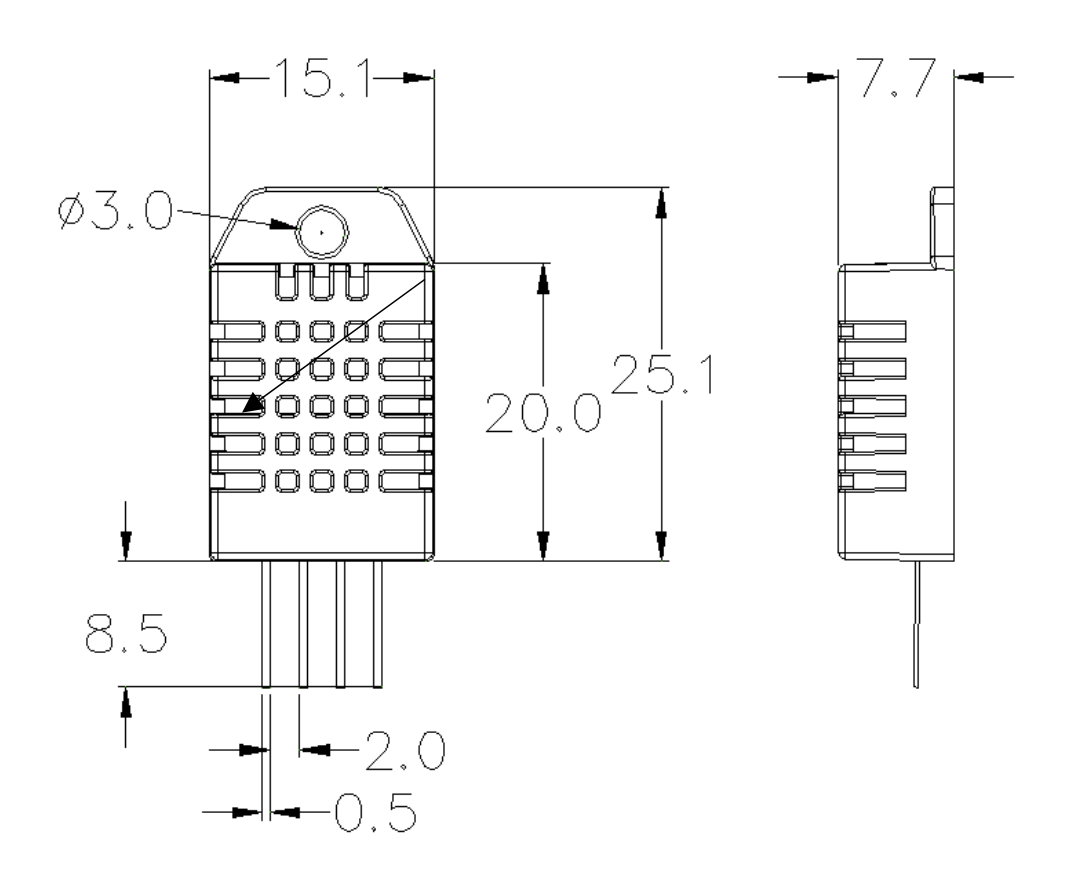
\includegraphics[width=.80\textwidth]{assets/dht-22.png} 
  \caption{Dimensões em milímetros do sensor DHT-22 (Retirado de \cite{datasheetDHT22}).}
  \label{fig:dht-22} 
\end{figure}

% ---
\section{Protocolos de comunicação}
\label{fund:protocolos}

% ----
\subsection{LoRa}
\label{fund:lora}
A tecnologia Long Range, LoRa, é uma forma de comunicação sem fio, semelhante ao Wi-Fi e ao Bluetooth, que permite um longo alcance de comunicação com baixo custo. O raio de comunicação sem fio utilizando o LoRa, dependendo do dispositivo selecionado, pode alcançar quilômetros de distância.

Embora o LoRa tenha sido fundamentalmente desenvolvido pela Semtech Corporation, o padrão imposto pelo LoRa permitiu que muitas empresas utilizassem para diversos projetos com um custo benefício satisfatório, aumentando o ecossistema e ganhando um envolvimento significativamente maior, uma variedade maior de produtos e um aumento geral no uso e aceitação. 

A baixa potência e os recursos de longo alcance significam que os pontos finais podem ser implantados em uma ampla variedade de locais, e ainda têm a capacidade de se comunicar com o gateway, que pode receber informações de vários LoRa e enviar para um servidor, por exemplo, e processar dados.

O LoRa em si diz respeito à camada física, sendo que a camada lógica é chamada de LoRaWAN, que é um protocolo usado pelo LoRa para comunicação entre pontos de conexões de um end-node para envios de informações do sistema.

\todo{falar do end-nodes e gateway}

% Referencias
% - https://www.profissionaisti.com.br/2017/11/iot-protocolo-lorawan-e-principais-placas-de-desenvolvimento-lora/
% - https://lora-alliance.org/sites/default/files/2018-07/lorawan1.0.3.pdf

% ----
\subsection{Wi-Fi}
\label{fund:wifi}

% ---
\section{Plataforma de prototipagem}
\label{fund:plataforma-proto}

% ---
\section{Servidor}
\label{fund:servidor}

% ----
\subsection{Node.js}
\label{fund:node}

% ----
\subsection{InfluxDB}
\label{fund:influxdb}
O InfluxDB é um banco de dados que armazena series temporais (\textit{data series database}), ou seja, sua chave é o tempo e sua forma de armazenagem de dados é em ordem cronológica. Ele foi projetado para lidar com grandes cargas de escrita e consulta, perfeita para armazenar dados em tempo real, como monitoramento de DevOps, métricas de aplicativos, big data e dados de sensores da IoT \cite{giacobbe2018implementation}. De forma geral, séries temporais acabam se tornando gráficos em função do tempo em um determinado período, por exemplo a temperatura de um freezer ao decorrer do dia, podendo assim ver facilmente a máxima, a minima e suas variações. Esses dados podem ser também coletados e feito uma analise mais complexa usando qualquer ferramente estatística, dependendo da sua necessidade.

O InfluxDB é composto por \textit{databases} (bancos de dados), \textit{measurements} (medições), \textit{fields} (campos) e \textit{tags}. Podemos representar essa estrutura como conjuntos como podemos ver na figura \ref{fig:influxdb-struct}, no InfluxDB é possível ter inúmeros \textit{databases}, onde cada \textit{database} contém suas \textit{measurements} que são tabelas de dados correspondente a algum dado em específico, por exemplo, se tivermos 2 sensores que coletam dados diferentes, cada sensor viraria um \textit{measurement}, e cada \textit{measurement} é composto  de dois tipo de atributos, os \textit{fields}, onde ficam os dados da sua medida, e as \textit{tags}, que são campos de dados que diferem \textit{fields} por serem campos indexáveis, feitos exclusivamente para realizar buscas, por exemplo, é comum adicionar uma \textit{tag} que seja um identificador do dispositivo que coletou esse medida.

\begin{figure}[H]
\centering
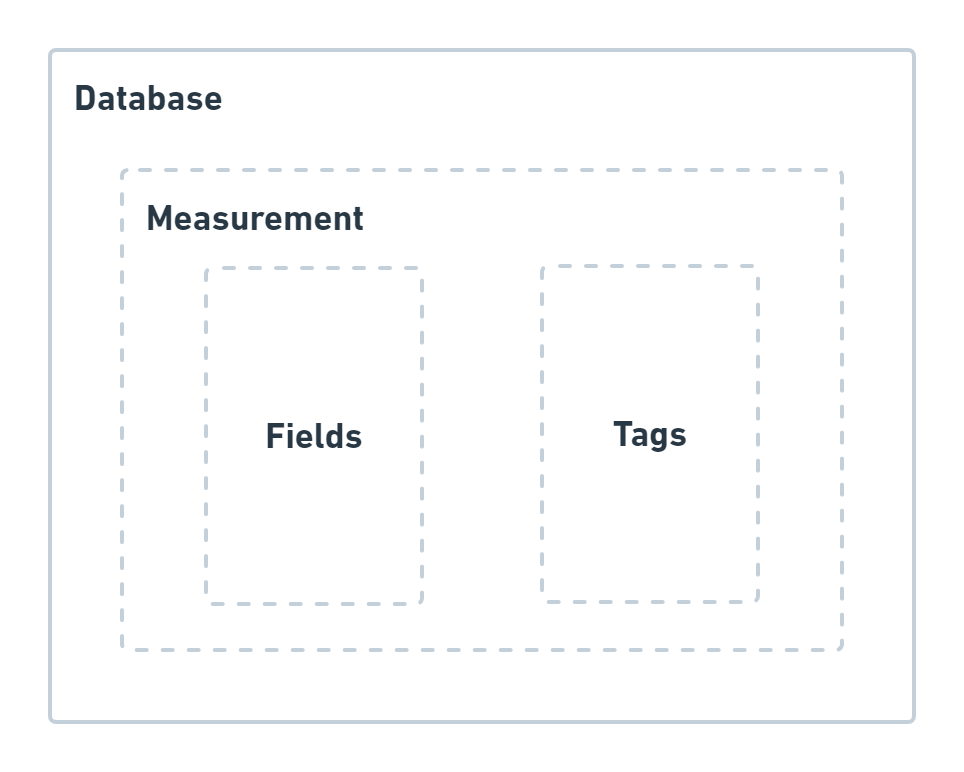
\includegraphics[width=.80\textwidth]{assets/influxdb-struct.png} 
\caption{Composição de um banco de dados do InfluxDB (Autoral).}
\label{fig:influxdb-struct} 
\end{figure}

% ----
\subsection{Docker}
\label{fund:docker}
Docker é uma plataforma \textit{open source}, desenvolvida utilizando a linguagem de programação GO pela Google com o objetivo de criar facilmente  ambientes isolados (containers) com um alto desempenho e que sejam portáteis, sendo uma opção em relação as virtualizações. Desta maneira, é possível, por exemplo, criar inúmeras aplicações usando as mesmas tecnologias, cada uma em um \textit{container} diferente e nenhuma vai interferir na outra, e todas na mesma máquina, e se for preciso replicar em outra máquina, é possível criar uma imagem do container e instalar o mesmo ambiente nesta outra máquina.

Em comparação com as virtualizações, os containers não precisam de um sistema operacional, apenas o essencial para executar determinada função. Dessa forma, os containers conseguem ter um controle maior, consomem menos recursos, ganham uma maior flexibilidade e uma manutenibilidade. Podemos ver a comparação entre virtualização e containers na figura abaixo.

\begin{figure}[!ht]
\centering
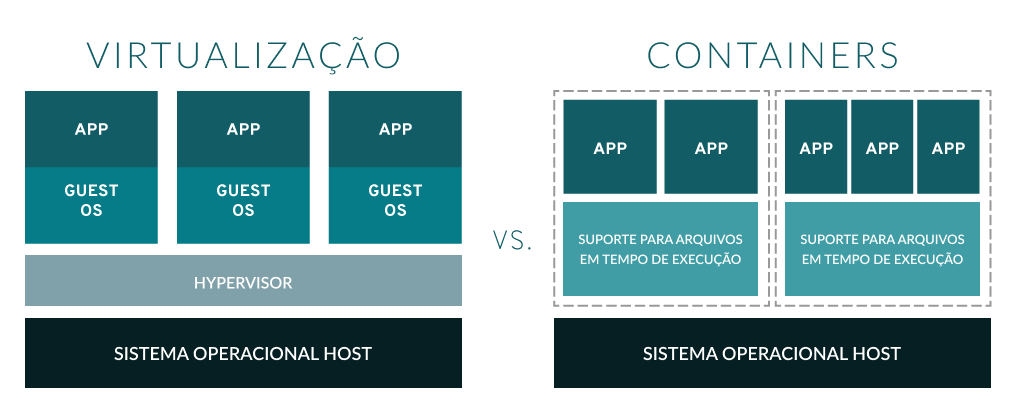
\includegraphics[width=.80\textwidth]{assets/virtualization-vs-containers.png} 
\caption{Comparação entre o modelo de virtualização e modelo de containers (Adaptada de Red Hat \cite{redhat2020Containers}).}
\label{fig:virtualization-vs-containers}
\end{figure}

% Referencias
% - https://www.opservices.com.br/o-que-e-docker/
% - https://www.meupositivo.com.br/panoramapositivo/container-docker/
% - https://www.treinaweb.com.br/blog/no-final-das-contas-o-que-e-o-docker-e-como-ele-funciona/

% % ---
\section{Aplicativo movel}
\label{fund:app}

% ----
\subsection{React Native}
\label{fund:react-native}

% ---
\section{Trabalhos Relacionados}
\label{fund:trabalhos-relacionados}